\documentclass[a4paper]{scrreprt}

\usepackage[ngerman]{babel}
\usepackage[utf8]{inputenc}
\usepackage[T1]{fontenc}
\usepackage{lmodern}

\usepackage[german,linesnumbered,algoruled,longend,vlined]{algorithm2e}
\DontPrintSemicolon
\SetArgSty{}
\SetKw{KwOr}{or}
\SetKw{KwAnd}{and}
\SetKw{KwNot}{not}
\setlength{\algomargin}{3ex}

\usepackage[fixlanguage]{babelbib}
% \selectlanguage{ngerman}
\setbibliographyfont{title}{}
\setbibliographyfont{jtitle}{}
\setbibliographyfont{btitle}{\emph}
\setbibliographyfont{stitle}{\emph}
\setbibliographyfont{journal}{\emph}

\usepackage{amsmath}
\usepackage{amsfonts}
\usepackage{amssymb}
\usepackage{amsthm}

\usepackage{graphicx}
\usepackage[bookmarks,bookmarksnumbered]{hyperref}
\usepackage[font=small,format=hang,labelfont=bf,figurename=Abb.,tablename=Tab.]{caption}
\usepackage{subcaption}
\usepackage{enumerate}

\newtheorem{satz}{Satz}[chapter]
\newtheorem{lemma}[satz]{Lemma}
\newtheorem{beobachtung}[satz]{Beobachtung}
\newtheorem{folgerung}[satz]{Folgerung}
\newtheorem{korollar}[satz]{Korollar}
\theoremstyle{definition}
\newtheorem{definition}[satz]{Definition}
\newenvironment{beweis}{\begin{proof}}{\end{proof}}

\graphicspath{{abbildungen/}}

% Eigene Commands:
\newcommand{\degree}{\ensuremath{^\circ}}
\newcommand{\go}{glatt-or\-tho\-go\-nal}
\newcommand{\Go}{Glatt-or\-tho\-go\-nal}
\newcommand{\Epsilon}{\mathcal{E}}
\newcommand{\N}{\mathbb{N}}


\begin{document}
%%%%%%%%%%%%%%%%%%%%%%%%%%%%%%%%%%%%%%%%%%%%%%%%%%%%%%%%%%%%%%%%%%%%%%%%%%
%%%%%%%%%%%%% Bitte nur ab hier Änderungen vornehmen %%%%%%%%%%%%%%%%%%%%%

%% hier Titel und Autorennamen eintragen

\subject{Bachelorarbeit}
\title{Implementierung eines Algorithmus\\ für das glatt-orthogonale Zeichnen \\ planarer Graphen} % Geben Sie hier den Titel Ihrer Arbeit an.
\author{Bernhard Häussner} % Geben Sie Ihren Namen an. 
\date{Eingereicht am 14. April 2014 \\ Version \today} % TODO: Geben Sie das Abgabedatum an, entfernen Sie das Versionsdatum
\titlehead{Julius-Maximilians-Universität Würzburg\\
Institut für Informatik\\
Lehrstuhl für Informatik I\\
Effiziente Algorithmen und wissensbasierte Systeme}
\publishers{Betreuer:\\
Prof.\ Dr.\ Alexander Wolff\\
Dipl.-Inf.\ Philipp Kindermann} % Geben Sie den Namen des weiteren Betreuers and
\maketitle
\tableofcontents




% TODO: Was ist das: ? Datenstrukturen, Testdaten, Probleme

\chapter{Einleitung}


Das automatisierte Zeichnen von Graphen stellt eine Vielzahl von Herausforderungen. 
Eine Herangehensweise ist es, zunächst einfachere oder speziellere Graphen zu zeichnen. 
Dazu Teilt man die Graphen in Klassen ein, die eine Aussage machen über die Schwierigkeit, den Graphen zu zeichnen. 
In dieser Arbeit geht es um die Klasse der planaren Graphen. Sie zeichnen sich dadurch aus, dass sie sich ohne Kantenüberschneidung in einer Ebene zeichnen und sie haben nur polynomial viele Kanten. 

Eine Anwendung des  automatisierte Zeichnens planarer Graphen ist die computergestützte Erstellung von Layouts für Schaltkreis-Platinen. Hierbei werden Komponenten, wie integrierte Schaltkreise (Chips), als Knoten modelliert und die verbindenden Leiter als Kanten. Da die Leiter im Herstellungsprozesses  aus technischen Überlegungen nur entweder horizontal oder vertikal auf einem Gitter verlaufen können, beschränkt man sich hier auf orthogonale Layouts. Bei solchen orthogonalen Zeichnungen planarer Graphen können nur 4~Kanten je Knoten ohne Überdeckungen verbunden werden. Man nennt diese vier möglichen Richtungen Ports. Die Graphen, die sich so zeichnen lassen gehören zu der Klasse der 4-planaren Graphen: planare Graphen, deren maximaler Kontengrad~4 ist. Abhängig von der maximalen Anzahl~$k$ der Knicke in einer Kante in einem Layout, teilen wir es in die Klasse $OC_k$ ein. % TODO: OC-x knicke oder komponenten? check liu, brandes und smooth

Orthogonale Layouts wurden in der Vergangenheit auch aufgrund ihrer Praxisrelevanz stark verbessert. Sie sind zur Visualisierung von Graphen für Menschen (etwa für abstrahierte ÖPNV-Netze, Organigramme, UML-Diagramme) jedoch nur schlecht geeignet, da sie schnell unübersichtlich wirken. % TODO: Quelle?, Roberts et al.?
Natürlich kann Übersichtlichkeit nicht genau definiert werden; jedoch werden die harten 90\degree-Knicke in den Kanten, an denen sich horizontale und vertikale Abschnitte treffen, leicht mit Knotenpunkten verwechselt. Auch wirken sie eher technisch und deshalb für bestimmte Zielgruppen wenig ansprechend.

Um dieses Problem zu lösen, glättet man die Knicke mit Kreisbögen. Man redet dann von glatt-orthogonalen Zeichnungen. Die Kreisbögen gehen tangential in die orthogonal verlaufenden geraden Abschnitte über. Die entstehenden Zeichnungen wirken übersichtlich, freundlich und ästhetisch, was für ansprechende Visualisierungen förderlich ist. Dadurch, dass die Kanten ansonsten trotzdem orthogonal verlaufen, bleibt die Komplexität der Layouts vergleichsweise gering. Man vergleiche hierzu etwa die in Handarbeit gefertigten Soziogramme des Künstlers Mark Lombardi (1951-2000), die u.a. aufgrund ihrer Runden Kanten eine gewisse Ästhetik erreichen, jedoch mangels orthogonaler Gitterstruktur wenig Systematik erkennen lassen. 

Bestehende Algorithmen zur automatisierten Erstellung glatt-orthogonaler Zeichnungen bauen auf bewährten Algorithmen für orthogonale Zeichnungen auf und erweitern diese so, dass genügend Platz für die abgerundeten Kanten bleibt, ohne dabei Kantenüberschneidungen einzuführen. Als Grundlage wählt man Algorithmen, welche die Anzahl der Knicke (auch pro Kante) in der entstehenden Zeichnung klein halten. 

Dabei müssen neue Herausforderungen angegangen werden. Ebenso wie Knicke in orthogonalen Zeichnungen für erhöhte Komplexität sorgen, sind in glatt-orthogonalen Zeichnungen Wechsel zwischen geraden und gekrümmten Abschnitten und zwischen Abschnitten aus Bögen mit unterschiedlichen Radien zu vermeiden. Gleichzeitig sollte die Fläche der Zeichnung nicht zu groß werden.

Es wäre trivial möglich, alle Kanten abzurunden, indem man Kreisbögen mit dem Radius der Gittergröße einfügt. So würden neben den Kreisbögen gerade Stücke über bleiben. Daher versucht man die Kreisbögen größer zu machen und so geschickt anzuordnen, dass möglichst wenige Wechsel zwischen verschiedenen Segmenten benötigt werden. Wir teilen die glatt-orthogonalen Zeichnungen in Abhängigkeit der maximalen Anzahl~$k$ von Segmentwechseln in einer Kante in die Klasse $SC_k$ ein. 

\section{Ziel}

Mit dieser Arbeit habe ich mir nun zur Aufgabe gemacht, einen solchen Algorithmus zum Erstellen glatt-orthogonaler Zeichnungen zunächst zu implementieren. Dazu werde ich den Algorithmus zunächst verständlich und so vollständig wie nötig erklären, um die zukünftige Verwendung von Verbesserung zu erleichtern. Damit der Leser ein umfassendes Bild des Algorithmus vermittelt bekommt, wird auch der Ausgangs-Algorithmus für orthogonale Layouts erklärt, sowie einige Hilfsroutinen. 

Die Implementierung ermöglicht es, für eine Reihe von Beispielgraphen \go e Layouts zu erstellen. Diese sollen die Nützlichkeit von glatt-orthogonalen Layouts unterstreichen und als Inspiration für die praktische Anwendung des Algorithmus dienen.

Dabei werden eventuelle Probleme aufgezeigt, die wiederum als Grundlage zur Verbesserung des Algorithmus dienen. 

\section{Struktur}


Der verwendete Algorithmus wird in Alam et al.~\cite{smooth-13} beschrieben. Er basiert auf orthogonalen
Layouts, welche mit dem Algorithmus von Biedl und Kant~\cite{biedl+kant-98} bzw. Liu et al.~\cite{liu+etal-98} erstellt
werden.

Diese Algorithmen werden zunächst noch einmal in ihrer Gesamtheit erklärt. Dabei werden die
verwendeten Definitionen genannt und die Notationen eingeführt. Die nötigen Datenstrukturen
werden konkretisiert und gelöste Teilprobleme erörtert. Daraufhin wird auf die Implementierung eingegangen und welche Besonderheiten sowie Herausforderungen hierbei zu
beachten waren. 

Im Anschluss wird die Implementierung mit verschiedenen Testdatensätzen kontrolliert. Anhand
der Ausgaben auf den Testdaten werden Schwachstellen des Verfahren identifiziert. 
Zuletzt werden noch einige Verbesserungsmöglichkeiten diskutiert, wie das Ergebnis
optimiert werden kann, im Hinblick auf Komplexität und Platzbedarf.

% TODO: Verweise auf Abschnitte, jeweils NACH der Beschreibung des Abschnitts







\chapter{Übersicht und Grundlagen}

In diesem Abschnitt sollen einige Grundlagen definiert werden. Zu jedem Begriff gibt es eine knappe Definition und einige Anmerkungen zur Relevanz für den Algorithmus. So wird die Problemstellung im Verlauf dieses Abschnittes immer klarer und im nächsten Abschnitt kann der Algorithmus mit den definierten Grundlagen präzise beschrieben werden.

\section{Graphen}

Zunächst sollte natürlich definiert werden, was überhaupt visualisiert werden soll:

\begin{definition}
  Ein \emph{(ungerichteter) Graph} $G$ ist ein Tupel $(V, E)$ von Mengen, wobei $E \subset \mathcal{P}(V)$.
  Die $v \in V$ heißen \emph{Knoten}, die $e \in E$ \emph{Kanten}.
\end{definition}

Graphen bilden die Eingabe für die Zeichenalgorithmen. Die hier behandelten Graphen werden auch \emph{Netzwerkgraphen} genannt, sie beschreiben Verbindungen zwischen Elementen als Kanten zwischen Knoten. 

Zunächst liegt der Fokus auf ungerichteten einfachen Graphen, das bedeutet, es gibt zwischen zwei Knoten jeweils nur höchstens eine Kante und eine \emph{Schleife}, also eine Kante mit $|e| = 1$ kommt nicht vor.

Einfache Graphen können im Computer als \emph{Adjazenzmatrix} $(a_{i,j})$ dargestellt werden, mit $a_{i,j} = 1$ falls $\{v_i, v_j\} \in E$ und $0$ sonst. Hier wird jedoch $O(|V|^2)$ Speicherplatz verwendet. Für Graphen mit vergleichsweise wenigen Kanten eignet sich die Darstellung als \emph{Adjazenzliste} $A$ mit $A(v) = \{e \in E | v \in e\}$. Hierfür wird $O(|V| + |E|)$ Speicher benötigt. % TODO: genau Checken!!!

\section{Orthogonale Visualisierungen von Graphen}

Die Darstellung von einfachen Graphen für Menschen, die \emph{Zeichnung} oder \emph{Visualisierung}, besteht üblicherweise aus Punkten, also kleinen Kreisen, für jeden Knoten und Verbindungslinien für die Kanten. Die Überführung von einer Adjazenzliste in einer solche Darstellung nennt man das \emph{Zeichnen} von Graphen. Hierfür gibt es keine kanonische Vorgehensweise. Der umgekehrte Weg von der Zeichnung zur Adjazenzliste jedoch ist (bei geeigneten Zeichnungen) trivial zu lösen.

Für \emph{Multigraphen} mit mehreren Kanten zwischen zwei Knoten kommen Variationen der Zeichnungen für einfache Graphen in Frage, die solche Kanten als Bündel oder dicker darstellen. Sie sollen daher hier nicht behandelt werden und einfache Graphen werden im Folgenden kurz als Graphen bezeichnet.

\begin{figure}[h]
  \centering
  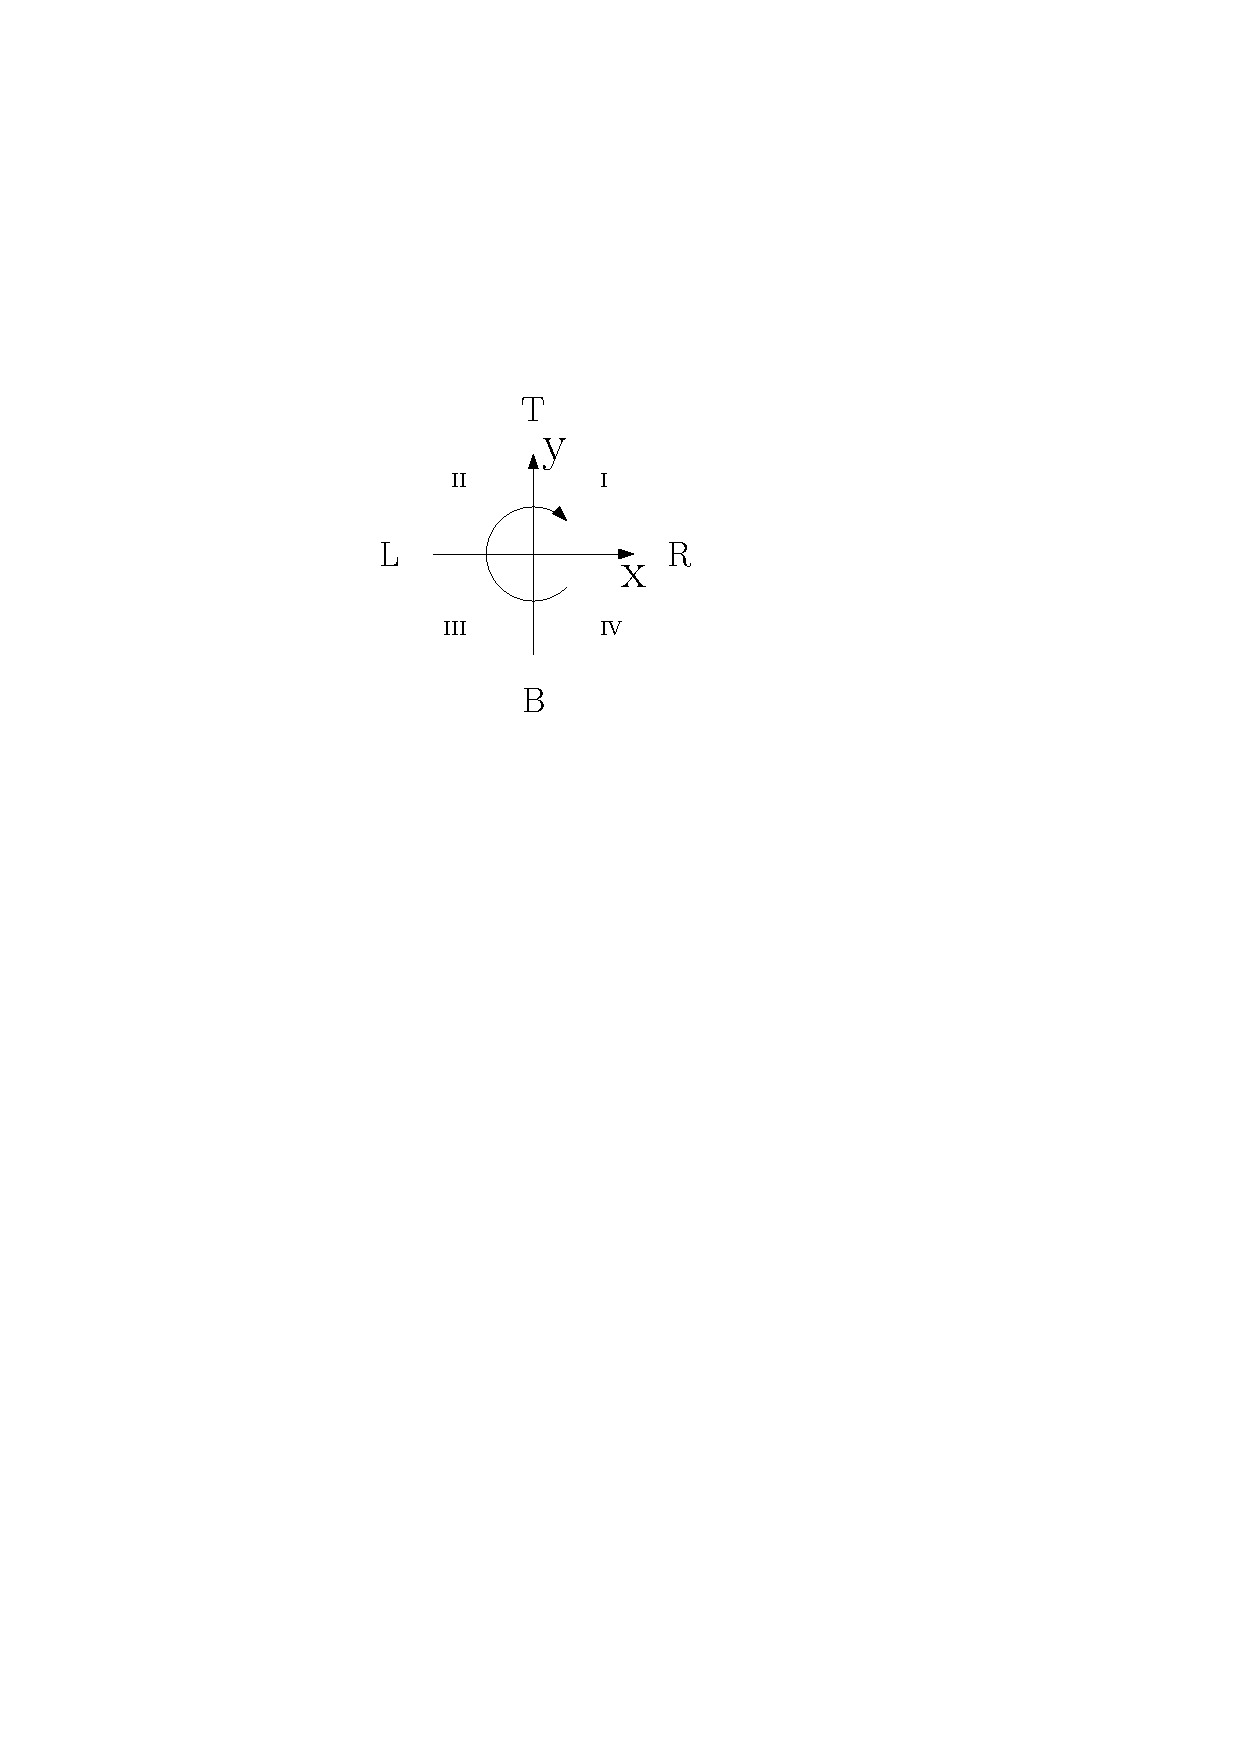
\includegraphics{koordinatengitter}
  \caption{Gezeichnet wird in eine Koordinatenebene. Hier wird die Anordnung der beiden Koordinaten-Achsen gezeigt, die Richtungen der Ports $\{\text{L, R, T, B}\}$, der Drehsinn der Anordnung im Uhrzeigersinn der Adjazenzlisten und die Quadranten $\{\text{I, II, III, IV}\}$.}
  \label{fig:coords}
\end{figure}

\begin{definition}
  Ein (zweidimensionales) \emph{Layout} $L$ über einer Menge $V$ ist eine Abbildung $L_V : V \to \N \times \N $. Ein \emph{Port} p ist eine Element der Menge \{\text{L, R, T, B}\}. Eine \emph{Portzuweisung} $P$ ist eine Abbildung $P: \{(v, e) \in V \times E | v \in e\} \to \{\text{L, R, T, B}\}$. Ein \emph{orhogonales Layout} ist ein 3-Tupel $(L_V,L_E,P)$ von Layouts $L_V$ und $L_E$ und einer Portzuweisung $P$.
\end{definition}

Die Hauptaufgabe eines Zeichenalgorithmus ist die Positionierung der Knoten auf einer Zeichenebene. Die berechnete Positionszuweisung heißt Layout. In einer \emph{geradlinigen Zeichnung} werden die Kanten als gerade Linien zwischen den Knoten gezeichnet. Hier bestimmt also die Position der Knoten vollständig das Aussehen der Kanten.

Bei orthogonalen Zeichnungen bestehen die Kanten aus horizontalen und vertikalen Segmenten entlang des Koordinatengitters der Zeichenebene. Damit gibt es eine Vielzahl von Möglichkeiten für das Aussehen der Kanten. Eine Möglichkeit, das Aussehen zu normieren, wäre es, immer zunächst den vollständigen horizontalen Weg am unteren Knoten und dann den vertikalen Weg nach oben zu zeichnen, sodass jede Kante L-förmig ist. Hierbei kommt es jedoch zu Überschneidungen, wenn beispielsweise zwei Kanten einen Knoten in die selbe Richtung verlassen. Überschneidungen sorgen für Zweideutigkeiten in der Zeichnung und sollen vermieden werden. Deshalb weißt man den Kanten an jedem Knoten einen Port aus der Menge $\{\text{L, R, T, B}\}$, also Links, Rechts, Top (oben) Bottom (unten) zu. Die Richtungen der Ports sind auch in Abbildung~\ref{fig:coords} zu erkennen.
\\

Das Zeichnen einer Kante $e$ eines Graphen $G = (V,E)$ in einem orthogonalen Layout $(L_V,L_E,P)$ kann nun so erfolgen: Von den von $L_V$ gegebenen Positionen der beiden Endknoten $v \in e$ wird eine Gittereinheit in der Richtung des Ports gezeichnet. Von diesen Positionen aus wird eine horizontale Linie in Richtung des von $L_E$ gegebenen Kantenorts gezeichnet. Die beiden Endpositionen werden mit einer vertikalen Linie verbunden. %% TODO: Proof?
\\

Es können jedoch immer noch Überschneidungen von Kanten an einem Knoten $v \in V$ auftreten, wenn die Ports kollidieren, wenn es also zwei Kanten $e_1, e_2 \in E$ mit $P(v, e_1) = P(v, e_2)$ gibt. Da es nur vier Ports gibt, können somit nur maximal vier Kanten mit einem Knoten verbunden sein.

\begin{definition}
  Die Anzahl $deg(v) = |\{e \in E | v \in e\}|$ ist der \emph{Grad} eines Knotens. Der Wert $deg(G) = \max_{v \in V}{deg(v)}$ eines Graphen $G = (V, E)$ ist der Grad des Graphen.
\end{definition}

Ohne Kanten-Überschneidungen an den Knoten können also nur Graphen mit Maximalgrad~4 gezeichnet werden. 

Es kann noch immer Überschneidungen bzw. Kreuzungen der Kanten an anderer Stelle geben.

\section{Zusammenhangs-Eigenschaften von Graphen}

\begin{definition}
  Ein \emph{Teilgraph} $G'$ eines Graphen $G=(V, E)$ ist ein Graph $G' = (V' \subset V, E' \subset E))$.
  Ein \emph{induzierter Teilgraph} $G_U$ eines Graphen $G=(V, E)$ über einer Menge $U \subset V$ ist der Kanten-Maximale Graph mit $G_U = (U , E' \subset E))$.
\end{definition}

Häufig werden nur Teile eines größeren Graphen betrachtet. % TODO: mehr?

\begin{definition}
  Ein \emph{Weg} ist ein Graph $G = (V, E)$ mit $V = \{v_1, v_2, \dots, v_n\}$ und $E = \{\{v_1, v_2\}, \{v_2, v_3\}, \dots, \{v_{n-1}, v_{n}\}\}$.
  Es gibt in einem Graphen $G = (V, E)$ einen Weg zwischen zwei Knoten $v_a, v_b \in V$, wenn es einen Teilgraphen von $G$, gibt, der ein Weg ist und $v_a$ und $v_b$ erhält.
  Ein Graph ist \emph{zusammenhängend}, falls es zwischen jeden zwei Knoten aus dem Graphen einen Weg gibt.
  Ist ein Graph nicht zusammenhängend, so nennt man die dispariten, maximalen zusammenhängenden Teilgraphen die \emph{Zusammenhangskomponenten}.
\end{definition}

Werden die Zusammenhangskomponenten einzeln gezeichnet, dann können sie unabhängig voneinander platziert werden: Zwei Zeichnungen von getrennten Zusammenhangskomponenten können beliebig nebeneinander gestellt werden. Ist in einer Teil-Zeichnung eine freie Fläche von der Größe einer anderen Teil-Zeichnung, könnten die kleine Zeichnung in der größeren Platz finden. Dies sind jedoch Optimierungsschritte, die unabhängig vom Zeichenalgorithmus der Komponenten sein können und auf die hier nicht weiter eingegangen wird.

\begin{definition}
  Man nennt zwei Knoten $v_\text{a}, v_\text{b} \in V$ in einem Graphen $G = (V, E)$ \emph{benachbart}, falls es eine Kante $e = \{v_\text{a}, v_\text{b}\}$ in $E$ gibt, und $v_\text{a}$ heißt in diesem Fall \emph{Nachbar} von $ v_\text{b}$ an $e$. 
\end{definition}

In dieser Sicht ist die reflexiv-transitive Hülle der Benachbart-Relation eine Äquivalenzrelation und ihre Äquivalenzklassen sind die Zusammenhangskomponenten des Graphen. %% TODO: Beweis?

\section{Zweifach-Zusammenhang und st-Ordnungen}

\begin{definition}
  Ein \emph{zweifach (knoten)zusammenhängender} Graph ist ein Graph $G=(V, E)$ für den jeder induzierte Teilgraph $G_{V \setminus v}$ für alle $v \in V$ zusammenhängend ist.
  Ist ein Graph $G=(V, E)$  nicht zweifach zusammenhängend, so nennt man die maximalen zweifach zusammenhängenden Teilgraphen die \emph{Zweifach-Zusammenhangskomponenten}. Die Zeugen $v \in V$, für die der induzierte Teilgraph $G_{V \setminus v}$ nicht zusammenhängend ist, nennt man \emph{Schnittknoten}. Kanten $e \in E$, für die $G' = (V, E \setminus e)$ nicht zusammenhängend ist, nennt man \emph{Brücken}.
\end{definition}

Ein Kreis ist ein zweifach zusammenhängender Graph, da durch Hinwegnahme eines Knotens ein zusammenhängender Weg entsteht. Ein Baum ist nicht  zweifach knotenzusammenhängend, da durch Hinwegnahme der Wurzel, die Kinder nicht mehr zusammenhängend sind.

Die Zweifach-Zusammenhangskomponenten eines Graphen bilden einen Baum.

Ein zweifach zusammenhängender Graph ist die Grundlage für eine weiteres Element das Zeichenalgorithmus:

\begin{definition}
  Eine \emph{$st$-Ordnung} eines zweifach zusammenhängenden Graphen $G = (V, E)$ und zweier Knoten $s, t \in V$ ist eine Anordnung aller Knoten $v_1, v_2, \dots, v_n \in V$, sodass $s = v_1$, $t = v_n$ und alle Knoten $v_i$ außer $s$ und $t$  einen Nachbarn $v_j$ mit $j < i$ und einen Nachbarn $v_k$ mit $k > i$ haben.
\end{definition}

Durch die $st$-Ordnung können die Knoten in eine Reihenfolge gebracht werden, in der sie der Algorithmus bearbeiten kann. Die $st$-Ordnung hat noch einige weitere Eigenschaften in planaren Graphen, die im nächsten Abschnitt besprochen werden.

\section{Planare Graphen}

%% TODO!!!



% Gerichtete Graphen, Grahp<=>Relation...

\section{Glatt-orthogonale Zeichnungen}

\cite{bekos-13}


\chapter{Algorithmus}

\section{Übersicht}

Zunächst werden nur zweifach knotenzusammenhängende Graphen gezeichnet, mittels Algorithmus~\ref{alg:biconnected}: Für den Graphen wird eine planare Einbettung und eine st-Ordnung bestimmt. Im nächsten Schritt wird ein orthogonales Layout berechnet, welches die Einbettung beibehält und die Knoten in der von der st-Ordnung vorgegebenen Reihenfolge platziert. Dieses orthogonale Layout wird dann verkleinert, wobei stufenförmige Kanten entfernt werden. Das fertige $OC_3$-Layout wird im letzten Schritt in ein $SC_2$-Layout umgesetzt.

\begin{algorithm}[ht]
  \SetKw{True}{true}
  \SetKw{False}{false}
  \caption{SmoothOrthogonalDrawBiconnected(Graph $G = (V,E)$)}
  \label{alg:biconnected}
  \Ein{4-planarer, zweifach knotenzusammenhängender Graph $G = (V,E)$}
  \Aus{$SC_2$-Layout von $G$}
  
  $\Epsilon \leftarrow$ PlanarEmbedding$(G)$ \;
  $St \leftarrow$ StOrdering$(G, \Epsilon)$ \;
  $O \leftarrow$ OrthogonalDrawing$(G,St,\Epsilon)$ \;
  $O' \leftarrow$ EliminateS-Shapes$(O)$ \;
  $\Gamma \leftarrow$ DrawSmoothEdges$(O')$ \;
  
  \Return $\Gamma$
\end{algorithm}


\section{Bestimmung einer planaren Einbettung}

% TODO

\cite{hopcroft+tarjan-74} \cite{patrignani-07} \cite{brandes-09}


\section{Ermitteln einer st-Ordnung}

Im nächsten Schritt wird eine \emph{st-Ordnung} berechnet, eine Reihenfolge der Knoten $v_1, \dots, v_n$, mit $s=v_1$ und $t=v_n$. Jeder Knoten (außer $s$ und $t$) soll mindestens einen Nachbarn mit einem höheren Index und mindestens einen mit einem niedrigeren Index haben. Da die Indizes paarweise verschieden sind, erhalten wir zudem einen gerichteten Graphen, wenn wir die ungerichteten Kanten so ausrichten, dass sie vom niedrigeren Index zum höheren verlaufen.\footnote {Umgekehrt könnten wir aus dem ungerichteten Graphen durch topologisches Sortieren eine st-Ordnung erhalten.}

Die st-Ordnung soll mir der planaren Einbettung kompatibel sein, d.h. wir wählen zwei Knoten $s$ und $t$ auf der Außenfacette. Damit haben wir günstige Reihenfolge für die Platzierung der Knoten bei der Berechnung des Layouts. 

Eine solche st-Ordnung lässt sich mit einer angepassten Tiefensuche und einer passenden Nachbearbeitung für jeden zweifach zusammenhängenden Graphen ermitteln. Ein Beweis in Form eines Linearzeit-Algortihmus findet sich bei Even und Tarjan~\cite{even+tarjan-75}, basierend auf vorherigen Resultaten (\cite{hopcroft+tarjan-74},~\cite{tarjan-72}).

\section{Erstellung eines $OC_3$-Layouts}

Für die Erstellung des $OC_3$-Layouts erhalten wir die Knoten in der Reihenfolge der st-Ordnung $v_1, \dots, v_n$. Durch die st-Ordnung erhalten wir zudem gerichtete Kanten und die Knoten haben somit einen Eingangsgrad und einen Ausgangsgrad, die sich, wegen der 4-Planariät, zu maximal 4 addieren. Außer $v_1$ und $v_n$ liegt bei den Knoten der Eingangsgrad und der Ausgangsgrad zwischen 1 und 3, da sie mindestens eine eingehende und mindestens eine ausgehende Kante haben. Die planare Einbettung $E$ gibt uns an jedem Knoten eine Reihenfolge der Kanten zu den adjazenten Knoten an. Ein- und Ausgehende Kanten liegen hierbei in zwei Abschnitten jeweils zusammen beieinander.

Am Ende bekommt jeder Knoten eine x-Koordinate (Spalte) und eine y-Koordinate (Zeile). Da wir die x-Koordinaten sonst häufig anpassen müssten, ordnen wir den Knoten zunächst nur Spalten zu. So können wir eine neue Spalte dazwischen einfügen, ohne die Koordinaten sämtlicher Knoten in den Spalten danach zu erhöhen. 

Neben den Knoten positionieren wir ebenso \emph{offene Kanten} in den Spalten: Alle Kanten, die gezeichnet werden, haben ein horizontales Segment, dessen Position in einer Spalte vorgemerkt wird. Das Ende der Kante wird hierbei noch nicht festgelegt. % TODO: Offene Kante definieren

Für die Erstellung des $OC_3$-Layouts werden die Knoten in der Reihenfolge der st-Ordnung auf einem Gitter platziert. Die y-Koordinate wird später nicht mehr benötigt und kann stets als $y(v_i) = i$ angenommen werden. Der erste Knoten wird in einer neuen, noch leeren Spalte platziert. Alle weiteren Knoten werden in der zugewiesenen Spalte der Kante an ihrem unteren Port platziert. Dazu müssen zunächst die Kanten den Ports zugewiesen werden.

Für die eingehenden Kanten werden je nach Eingangsgrad des Knotens folgende Ports verwendet: Unten (1-4), links (2-4), rechts (3,4), oben (4). Der obere Port wird also nur bei Eingangsgrad 4 verwendet, was nur bei der Senke $v_n$ vorkommen kann. Der untere Port wird nur bei Eingangsgrad 0 nicht verwendet, was nur bei der Quelle $v_1$ vorkommt. Den Ports werden dann die Kanten nach der Reihenfolge der planaren Einbettung in der Abfolge oben, links, unten, rechts zugewiesen.

Für die ausgehenden Kanten werden je nach Eingangsgrad des Knotens folgende Ports verwendet: oben (1-4), rechts (2-4), links (3,4), unten (4). Der untere Port wird also nur bei Eingangsgrad 4 verwendet, was nur bei der Quelle $v_1$ vorkommen kann. Den Ports werden dann die Kanten nach der Reihenfolge der planaren Einbettung in der Abfolge oben, links, unten, rechts zugewiesen. 
Für die Kante des oberen Ports wird ein Kantenort in der Spalte des Knotens vermerkt. Für die Kanten der Ports links und rechts werden jeweils Kantenorte in neuen Spalten links und rechts des Knotens vermerkt. Gibt es eine Kante im unteren Port, bekommt sie einen Knotenort in einer weiteren neuen Spalte weiter rechts. % TODO: schwammig

Ist der Algorithmus bei $v_n$ angekommen, sind alle Knoten eingebettet. Zuletzt nummerieren wir die Spalten durch und weisen den darin platzierten Knoten diese Nummer als x-Koordinate zu. 

\section{Eliminierung der stufenförmigen Kanten}

Das im letzten Schritt erstellte $OC_3$-Layout ist nicht sehr kompakt, da jeder Knoten in einer eigenen Zeile platziert ist. Außerdem sollen stufenförmige Kanten entfernt werden.

Zwei Knoten $v_i, v_k$ mit $i < k$ sind mit einer stufenförmigen Kante verbunden, wenn es eine Kante gibt, die am rechten Port von $v_i$ und am linken Port von $v_k$ ist. Solche Knoten nennen wir äquivalent bezüglich der Höhe und fassen gleich hohe Knoten in Äquivalenzklassen zusammen.

Diese Äquivalenzklassen verwenden wir als Knoten eines neuen gerichteten Graphen. Wir setzen eine gerichtete Kante zwischen zwei Äquivalenzklassen falls es eine gerichtete Kante zwischen zwei Knoten dieser Klasse gibt. Im so erhaltenen Graphen weisen wir der Klasse $\{v_1\}$ die Höhe $1$ zu. Dann weisen wir allen anderen Klassen jeweils die um 1 inkrementierte Höhe ihres höchsten Vorgängers zu, bis alle Klassen eine Höhe erhalten haben. Zuletzt weisen wir den Knoten die Höhe ihrer Klasse als y-Koordinate zu.

Offensichtlich kann es nun keine stufenförmigen Kanten mehr geben, da die entsprechenden Knoten in der gleichen Klasse sind.

\section{Konvertierung in ein $SC_2$-Layout}



\section{Entfernen von Überschneidungen im $SC_2$-Layout}



\section{Übertragen auf allgemeine 4-planare Graphen}

Algorithmus~\ref{alg:main}
% TODO: Textchen hierzu
% TODO: Ans Ende der Sektion schieben

\begin{algorithm}[ht]
  \SetKw{True}{true}
  \SetKw{False}{false}
  \caption{SmoothOrthogonalDraw(Graph $G = (V,E)$}
  \label{alg:main}
  \Ein{4-planarer Graph $G = (V,E)$}
  \Aus{$SC_2$-Layout von $G$}
  
  $G_1, \dots, G_n =$ BiconnectedComponents$(G)$ \;
  
  \For{$i\leftarrow 1$ \KwTo $n$}{
    $\Gamma_i \leftarrow$ SmoothOrthogonalDrawBiconnected$(G_i)$ \;
    MakeRightAngles$(\Gamma_i)$ \;
  }
  $\Gamma \leftarrow$ ConnectComponents$(\Gamma_1, \dots, \Gamma_n)$ \;
  \Return $\Gamma$
\end{algorithm}


\chapter{Implementierung}

\section{Software}

Für die Implementierung in der Programmiersprache \emph{Java} wurde, wo möglich, auf bestehende und bewährte Software-Grundlagen gesetzt.

Das Ausgangsformat, aus dem die Graphen eingelesen wurde, ist \emph{GraphML}~\cite{brandes+al-14}. Das freie Datenformat ist das Ergebnis von Bemühungen, ein Standardisiertes Format für das Speichern von Graphen zu schaffen. Es basiert auf XML, kann alle Arten von Graphen speichern und ist zudem um eigene Attribute erweiterbar, diese Erweiterungen können beim Einlesen übersprungen werden.

Die Eingabedaten für die Graphen stammen größtenteils aus den \emph{Rom-Testgraphen}\footnote{Erhältlich unter \url{http://www.graphdrawing.org/data/}}, eine Sammlung von verschiedensten Graphen mit 10 bis 100 Knoten im GraphML-Format. Für das schelle Erstellen von Testgraphen für einige Spezialfälle wurde der Grapheneditor \emph{yEd}\footnote{Erhältlich unter \url{http://www.yworks.com/de/products_yed_about.html}} von yWorks verwendet, der ebenfalls das GraphML-Format unterstützt und Graphen übersichtlich visualisieren kann.

Zum Einlesen der Graphen in Java und ihre Repräsentation im Speicher wurde \emph{JUNG}~\cite{jung}\footnote{Erhältlich unter \url{http://jung.sourceforge.net/}}, das \emph{Java Universal Network/Graph Framework}, verwendet. Es beinhaltet neben effizienten Implementierungen von verschiedenen Graphen, etwa gerichtete und ungerichtete, einige Algorithmen auf Graphen und Werkzeuge zur Visualisierung. Außerdem lassen sich damit GraphML-Dateien einlesen.

Die Ausgabe der fertigen Zeichnungen erfolgte im Vektorgrafik-Format des Editors \emph{Ipe}\footnote{Erhältlich unter \url{http://ipe7.sourceforge.net/}}. Das Format basiert auf XML und erhält Möglichkeiten für das Zeichnen von Punkten, Linien und Kreisbögen und vielem mehr. Der Vorteil gegenüber anderen Vektorformaten ist, dass sich \LaTeX-Beschriftungen in den Zeichnungen platzieren lassen und die Zeichnungen in PDF-Dateien konvertiert werden können. Die fertigen Zeichnungen können mit dem Ipe-Editor annotiert und weiter bearbeitet werden.

Zum Erstellen der Ipe-Dateien aus Java wurde die \emph{IpeDraw-Bibliothek}\footnote{Erhältlich unter \url{http://lamut.informatik.uni-wuerzburg.de/mediawiki/ipe7/index.php/JAVAtoIPE}} von Philipp Kindermann und Martin Fink verwendet.

Es wurden also Daten aus dem Rom-Testgraphen entnommen oder direkt in yEd erstellt, in Java mittels JUNG eingelesen, durch den Algorithmus visualisiert und mit der IpeDraw-Bibliothek als Vektorgrafiken ausgegeben, welche im Ipe-Editor betrachtet werden können oder in PDFs konvertiert werden.

\section{Schnitte finden}

\begin{figure}[h]
        \centering
        \begin{subfigure}[b]{0.2\textwidth}
                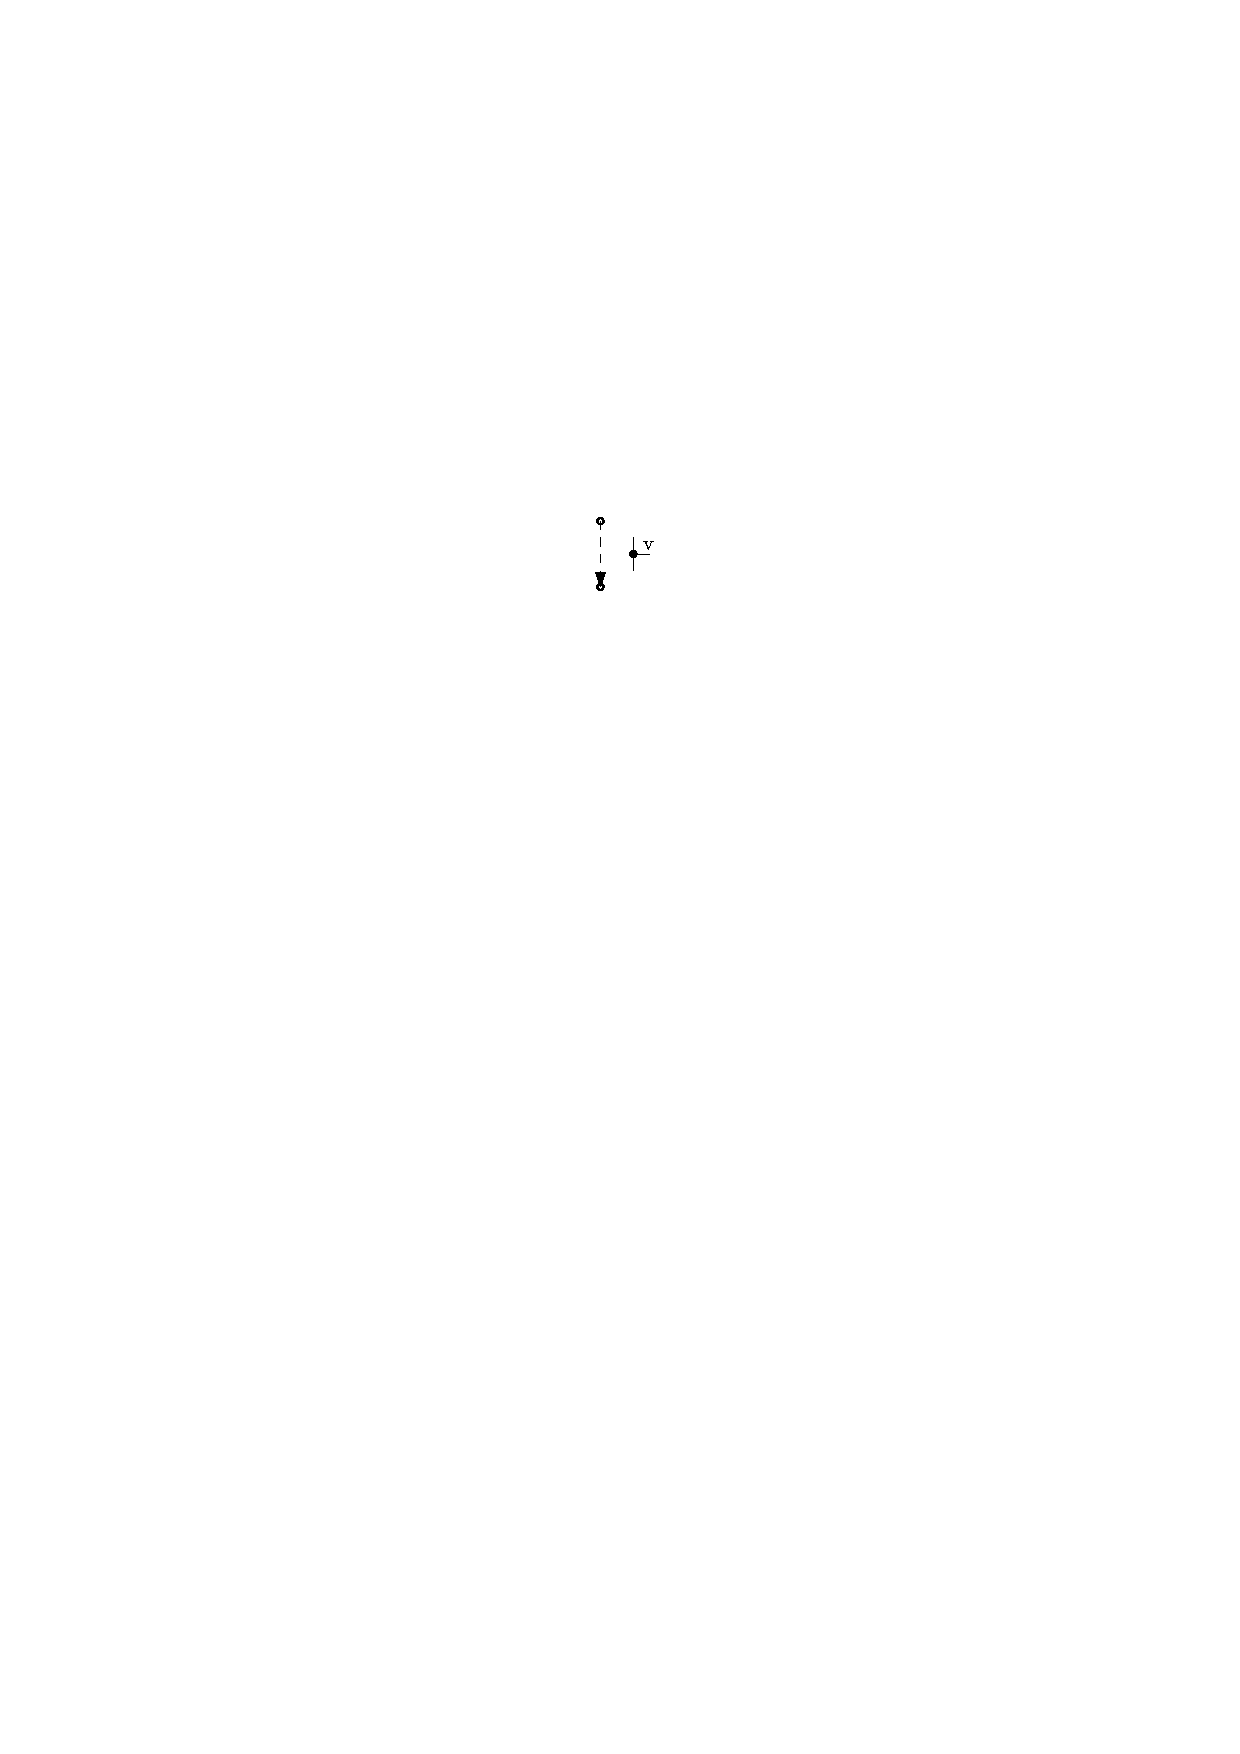
\includegraphics[width=0.5\textwidth]{schnitt_finden_top_none}
                \caption{Oberhalb,\\ keine Kante}
                \label{fig:cutfinding_top_none}
        \end{subfigure}%
        \quad
        \begin{subfigure}[b]{0.2\textwidth}
                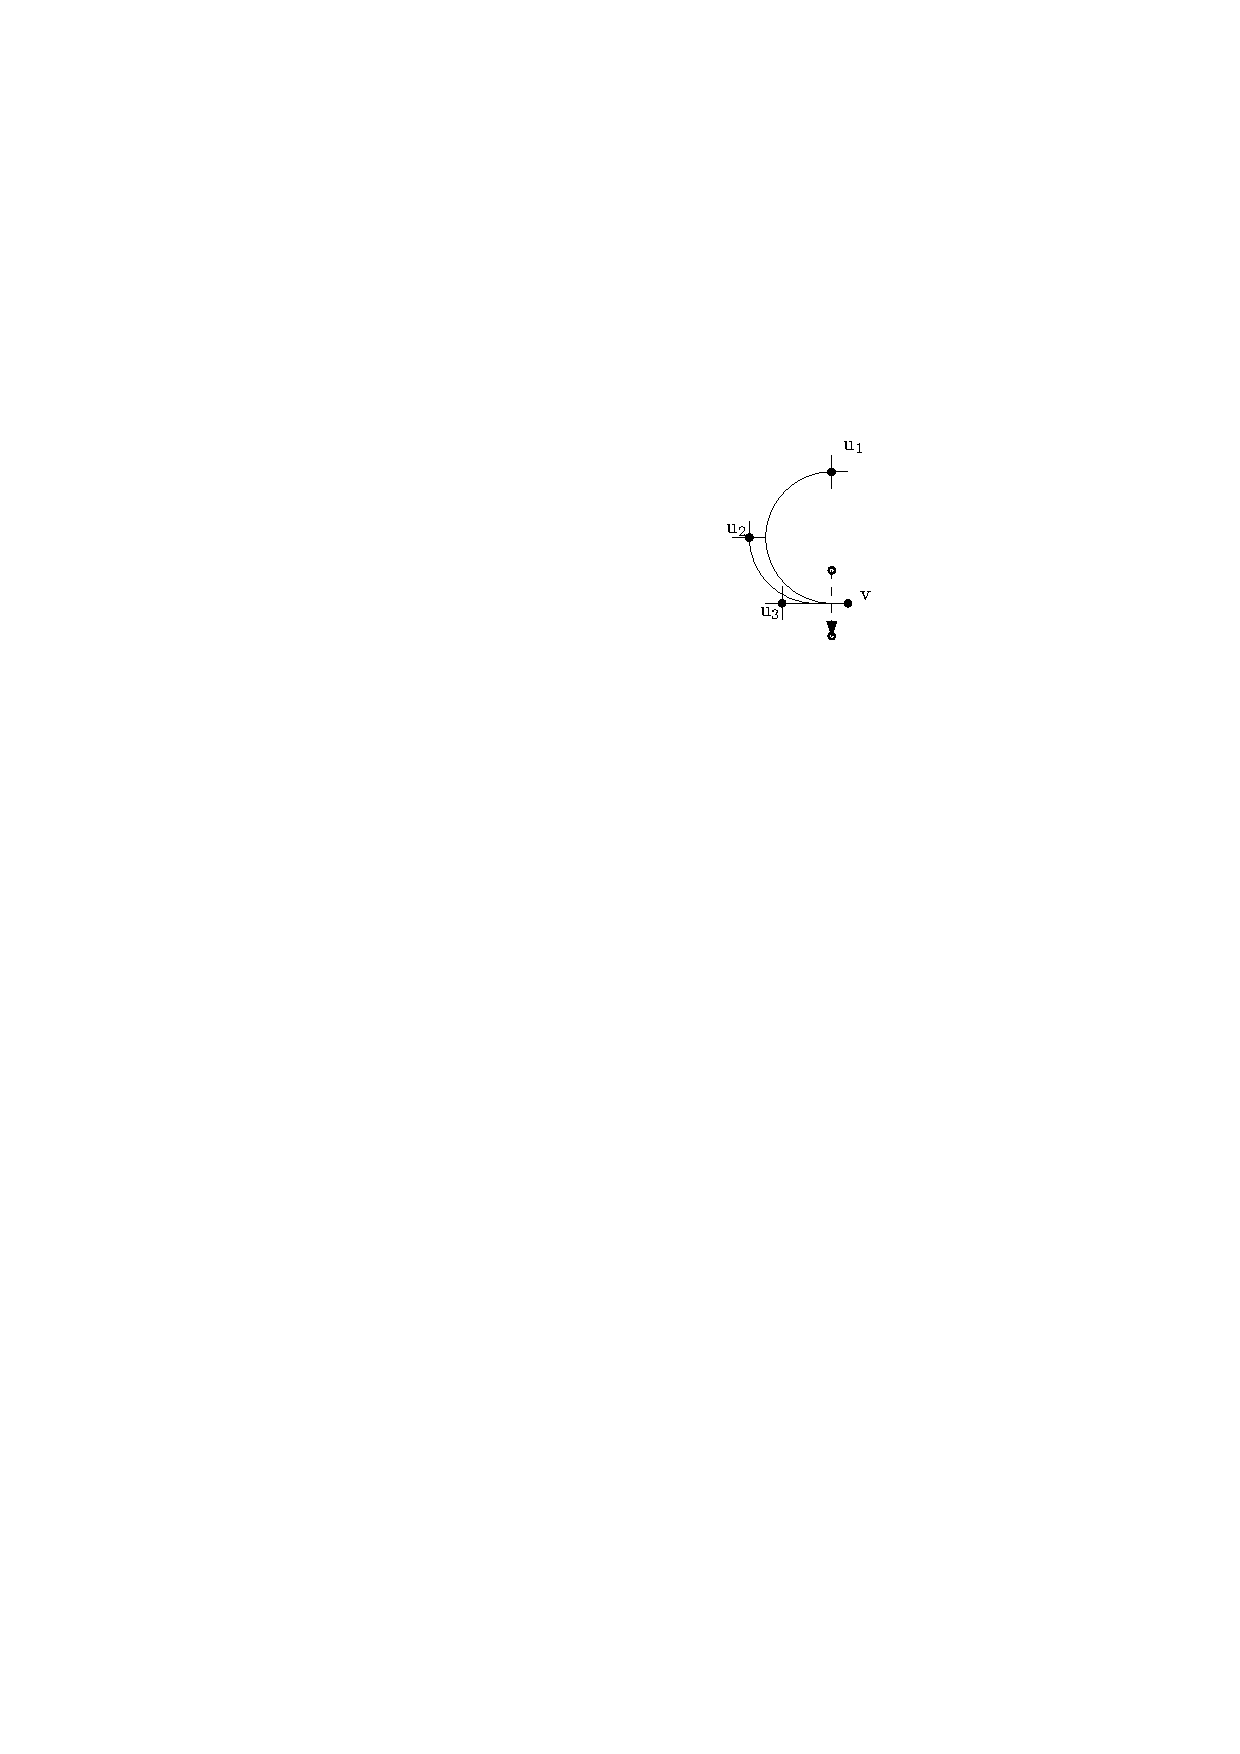
\includegraphics[width=\textwidth]{schnitt_finden_top_upwards}
                \caption{Oberhalb, Kante \\ nach oben}
                \label{fig:cutfinding_top_upwards}
        \end{subfigure}
        \quad
        \begin{subfigure}[b]{0.2\textwidth}
                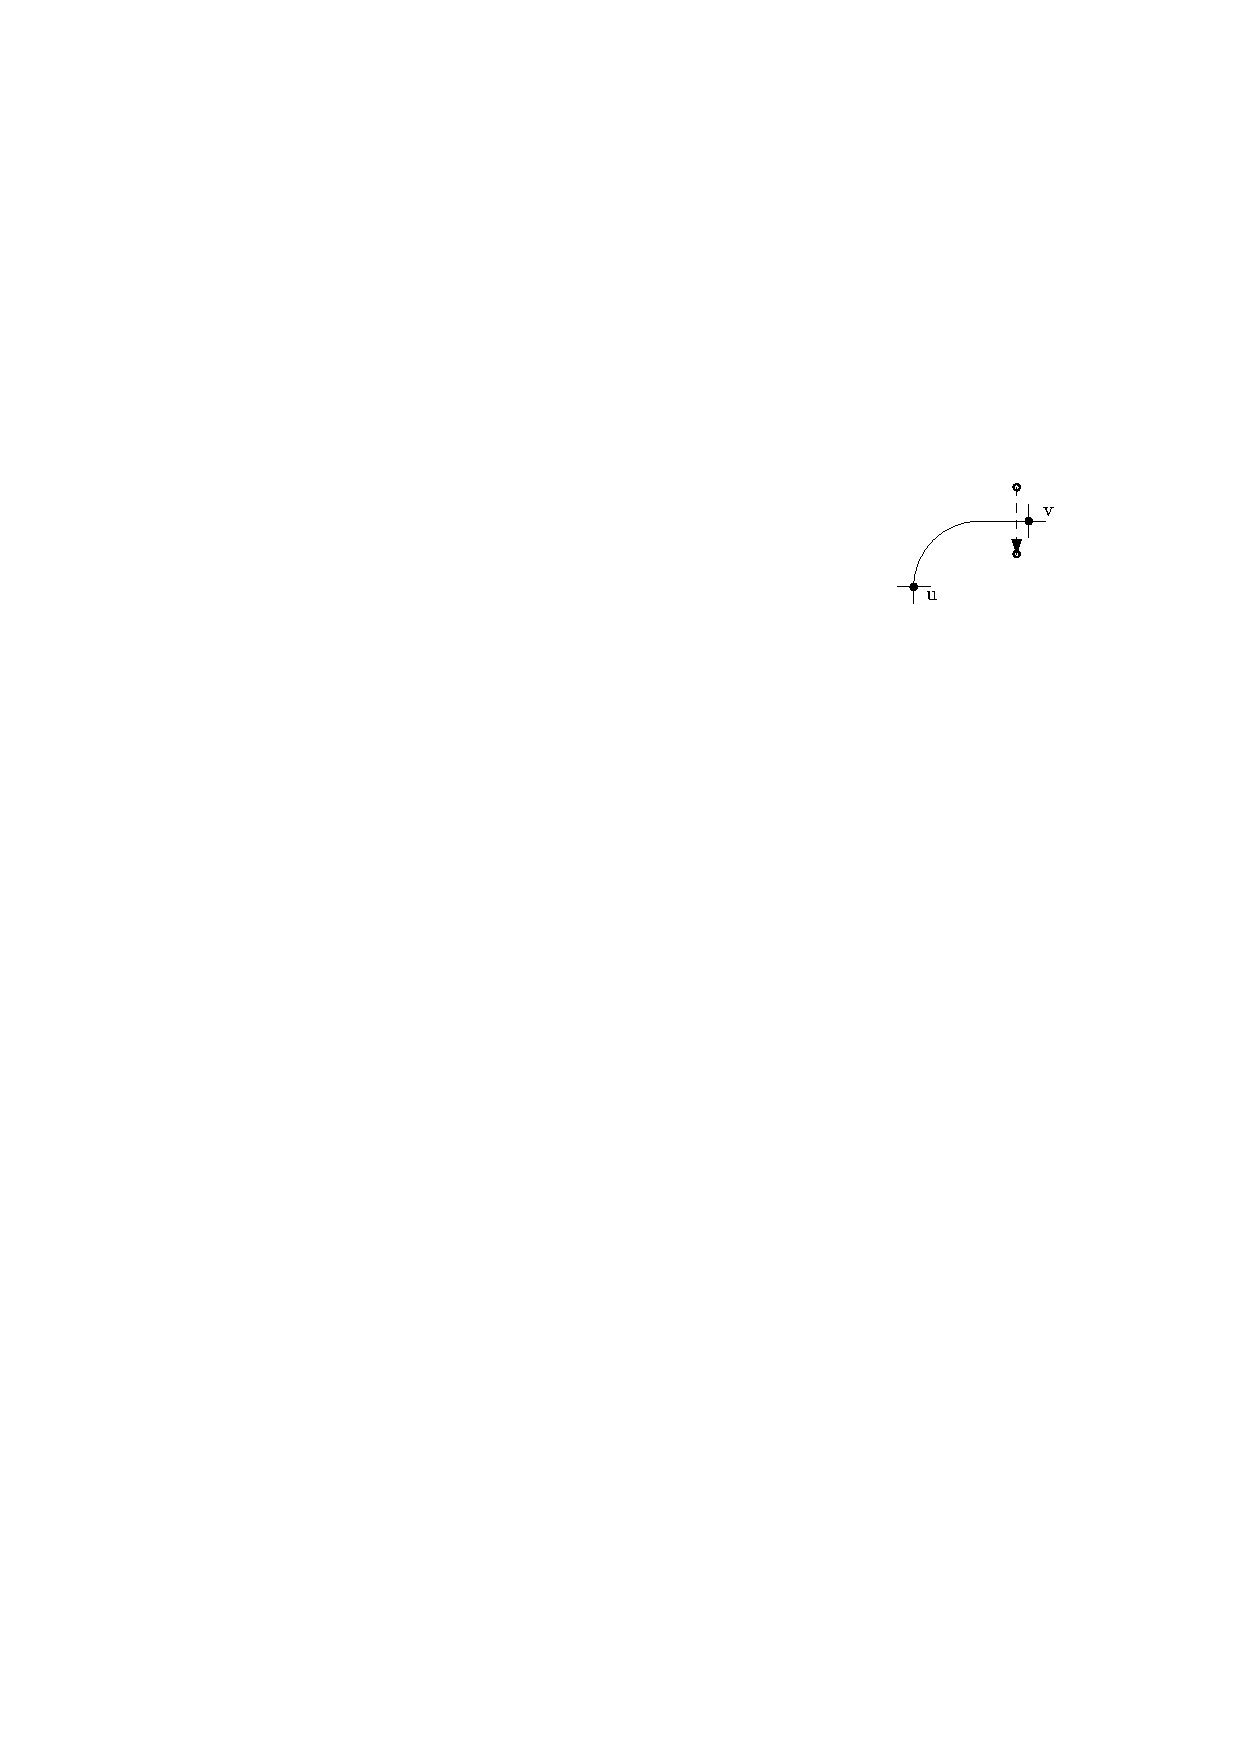
\includegraphics[width=\textwidth]{schnitt_finden_top_downwardsL}
                \caption{Oberhalb, L-Kante \\ nach unten}
                \label{fig:cutfinding_top_downwardsL}
        \end{subfigure}
        \quad
        \begin{subfigure}[b]{0.2\textwidth}
                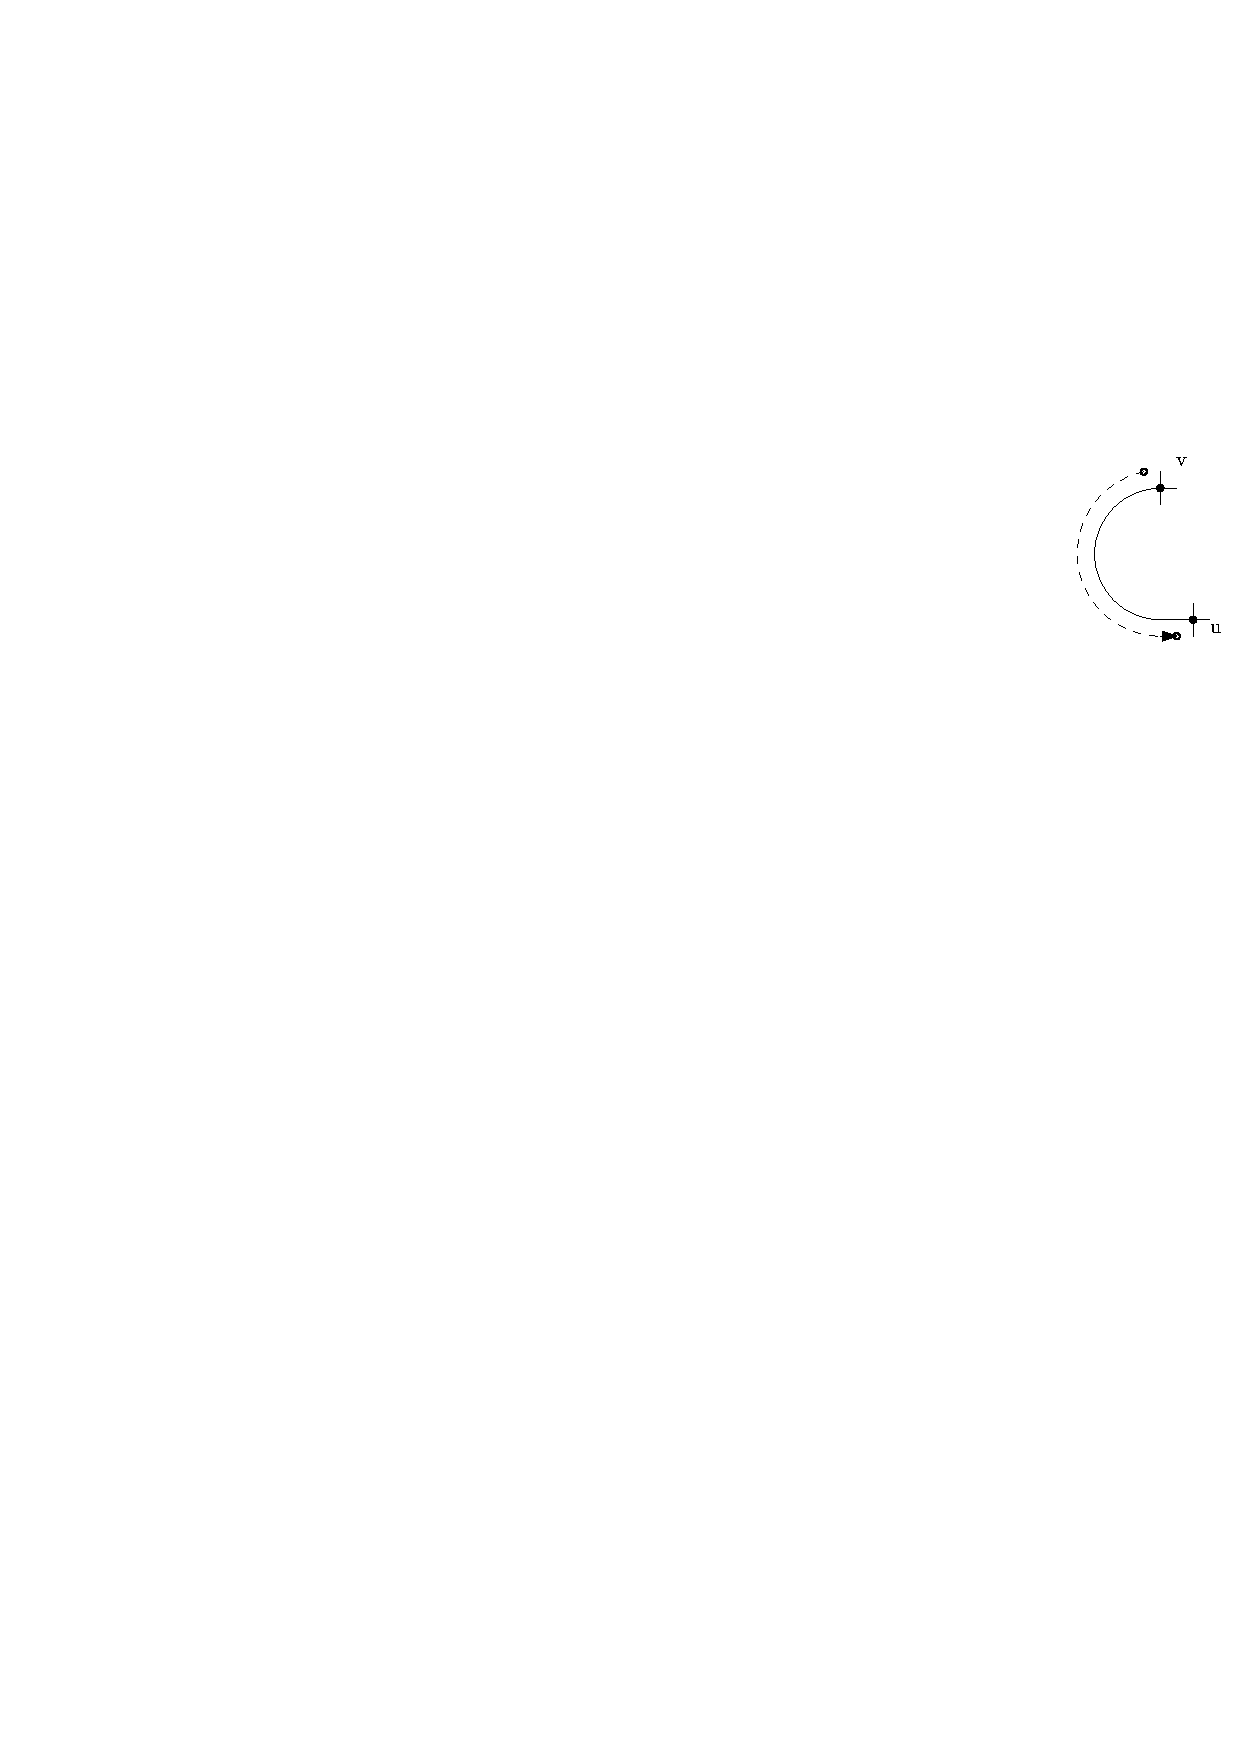
\includegraphics[width=\textwidth]{schnitt_finden_top_downwardsC}
                \caption{Oberhalb, \\ C-Kante \\ nach unten}
                \label{fig:cutfinding_top_downwardsC}
        \end{subfigure}
        \quad
        \begin{subfigure}[b]{0.2\textwidth}
                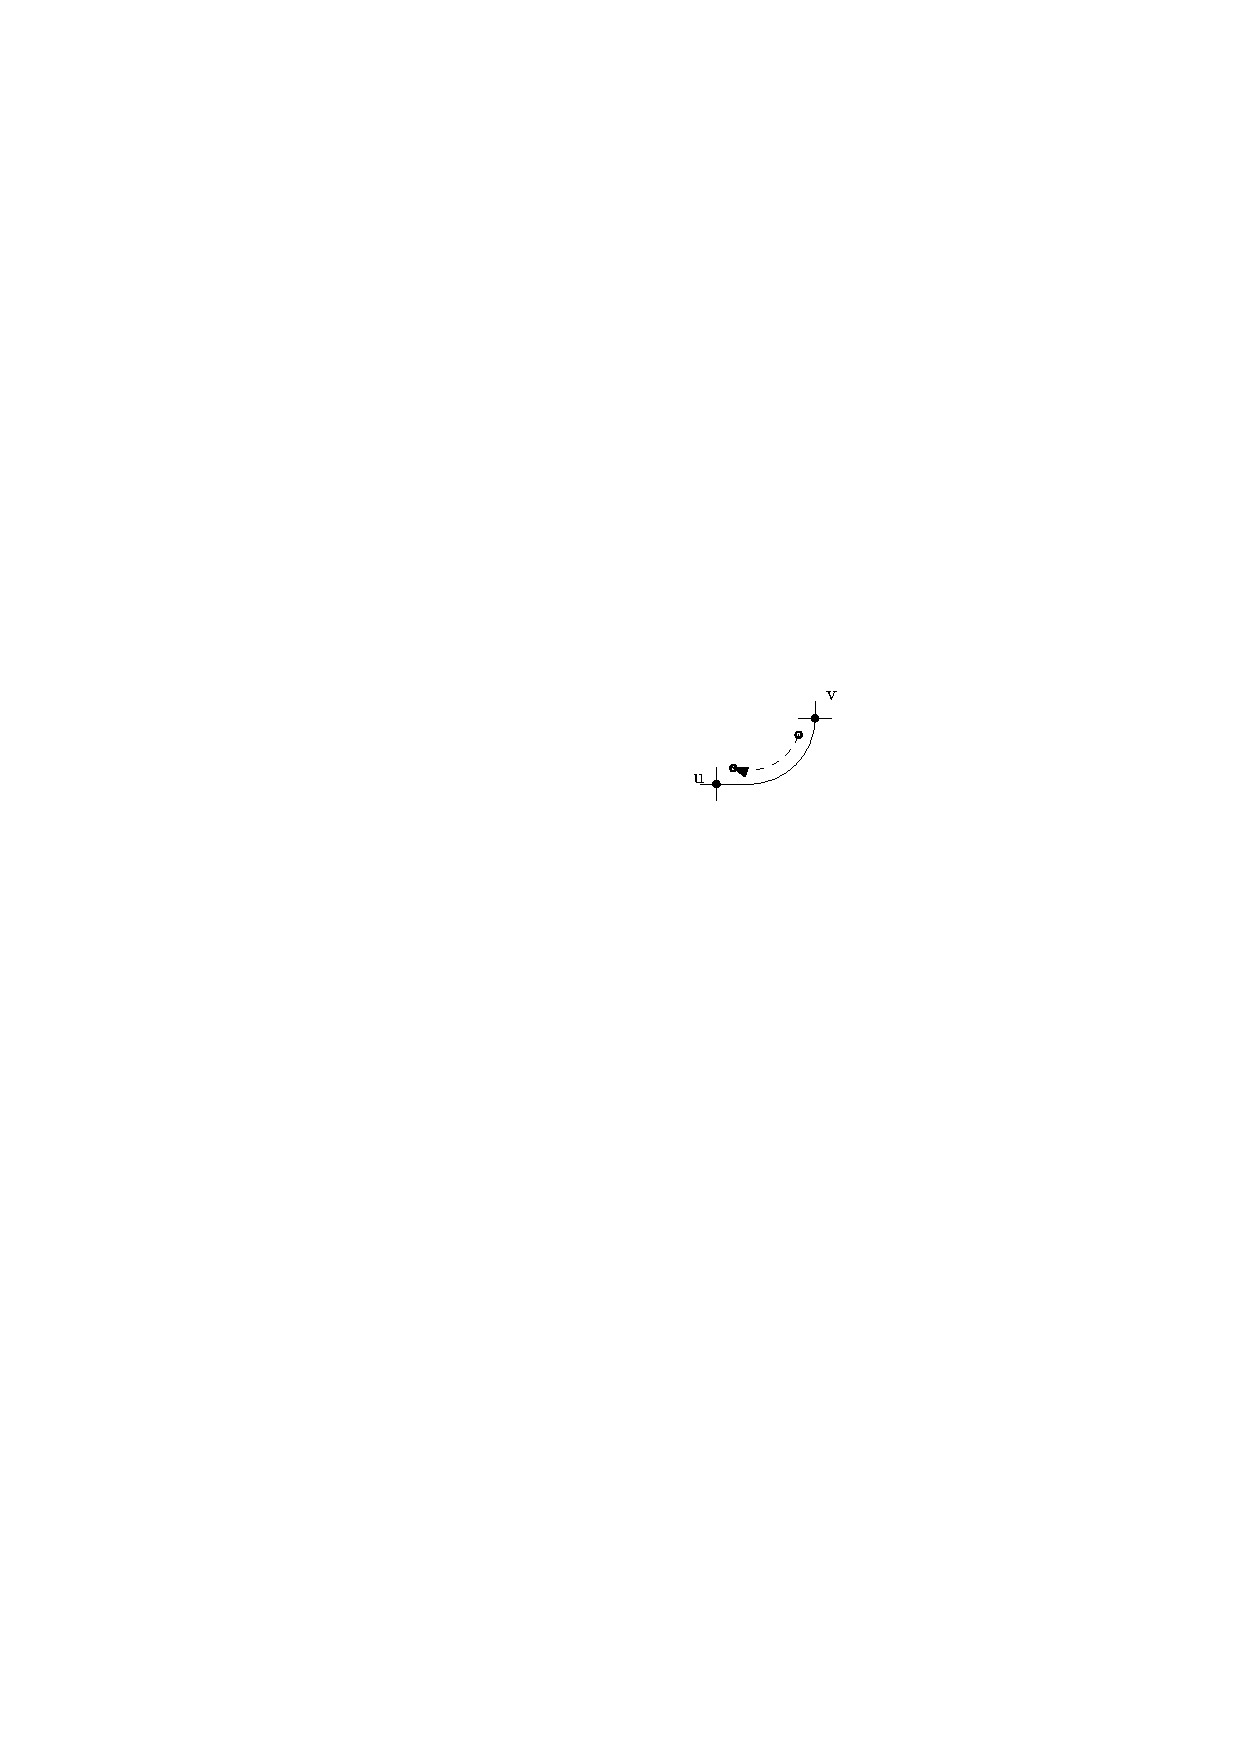
\includegraphics[width=\textwidth]{schnitt_finden_bot_aboveL}
                \caption{Unterhalb, über eine \\ L-Kante}
                \label{fig:cutfinding_bot_aboveL}
        \end{subfigure}
        \quad
        \begin{subfigure}[b]{0.2\textwidth}
                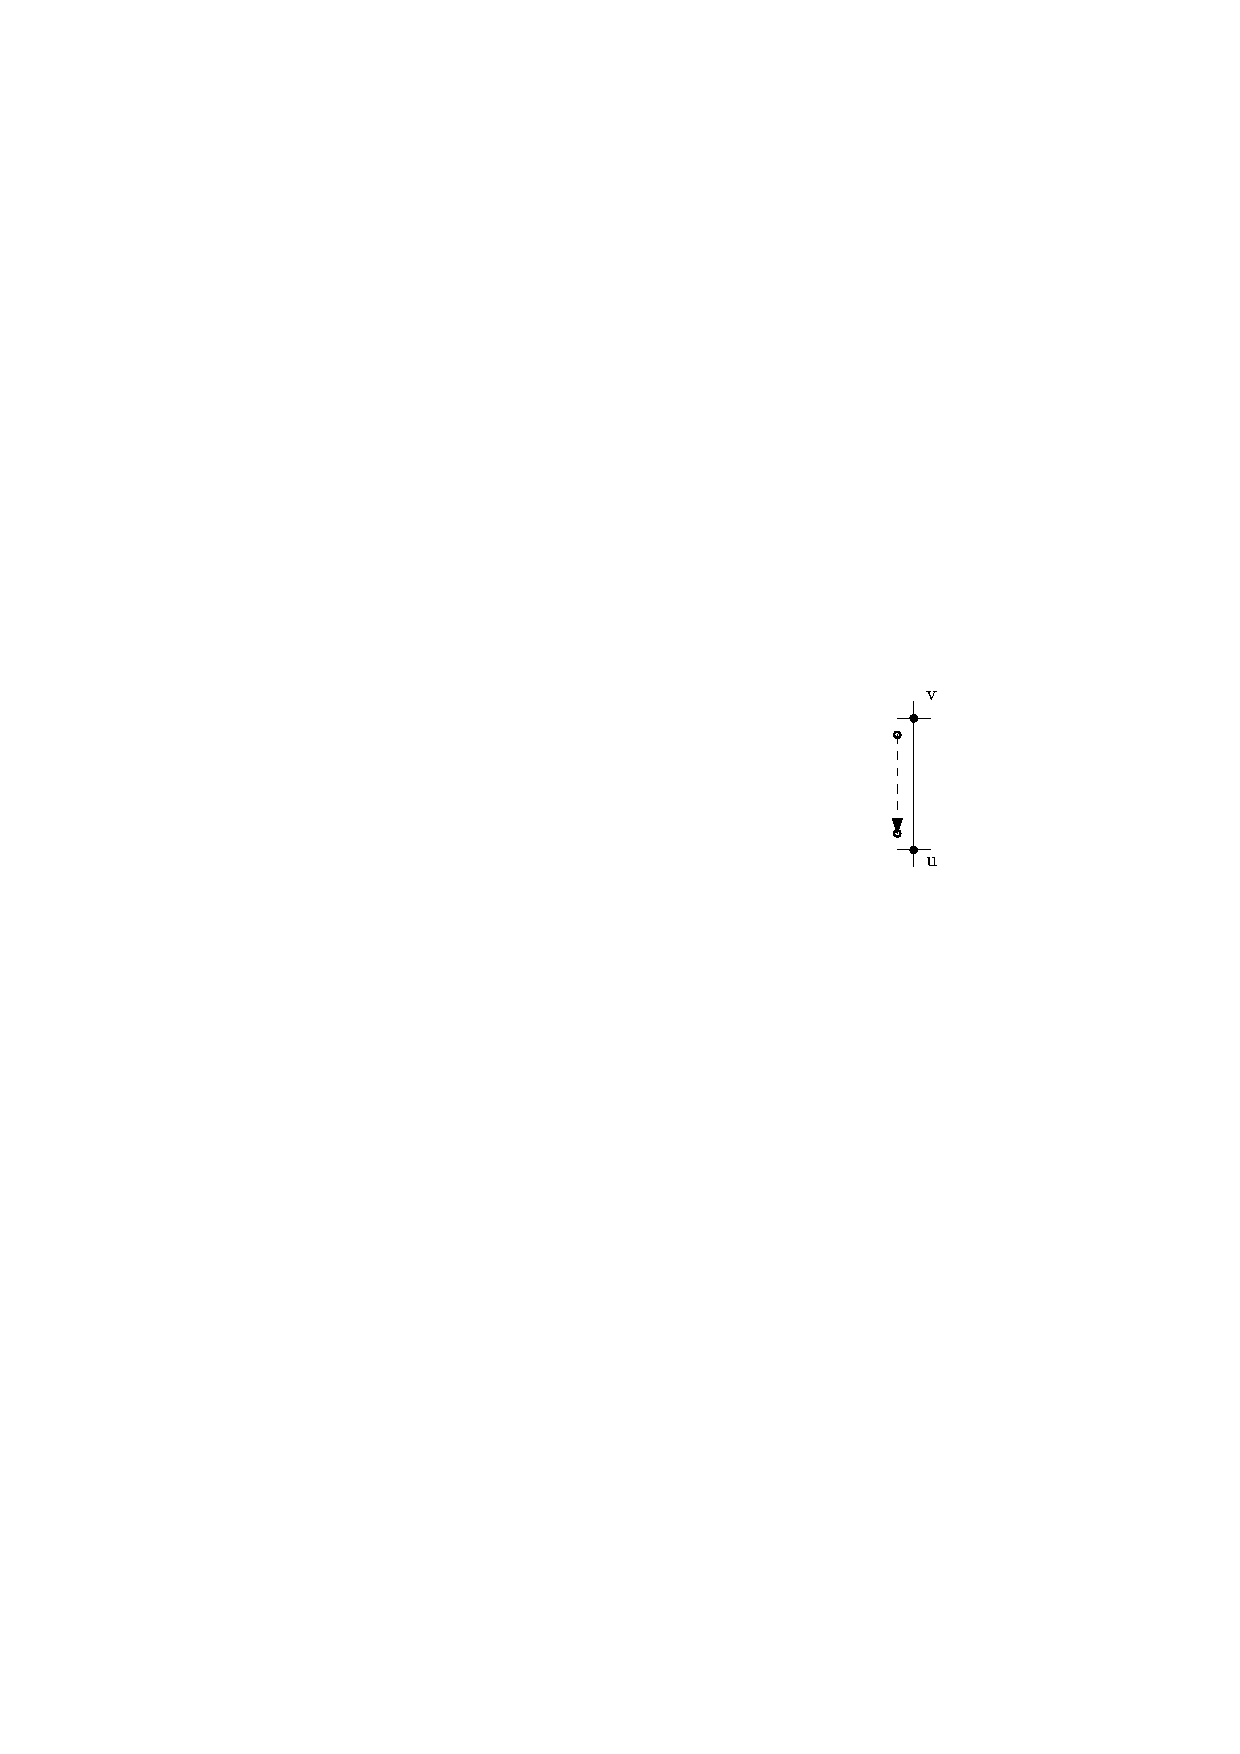
\includegraphics[width=0.25\textwidth]{schnitt_finden_bot_vertical}
                \caption{Unterhalb, entlang einer vertikalen Kante}
                \label{fig:cutfinding_bot_vertical}
        \end{subfigure}
        \quad
        \begin{subfigure}[b]{0.2\textwidth}
                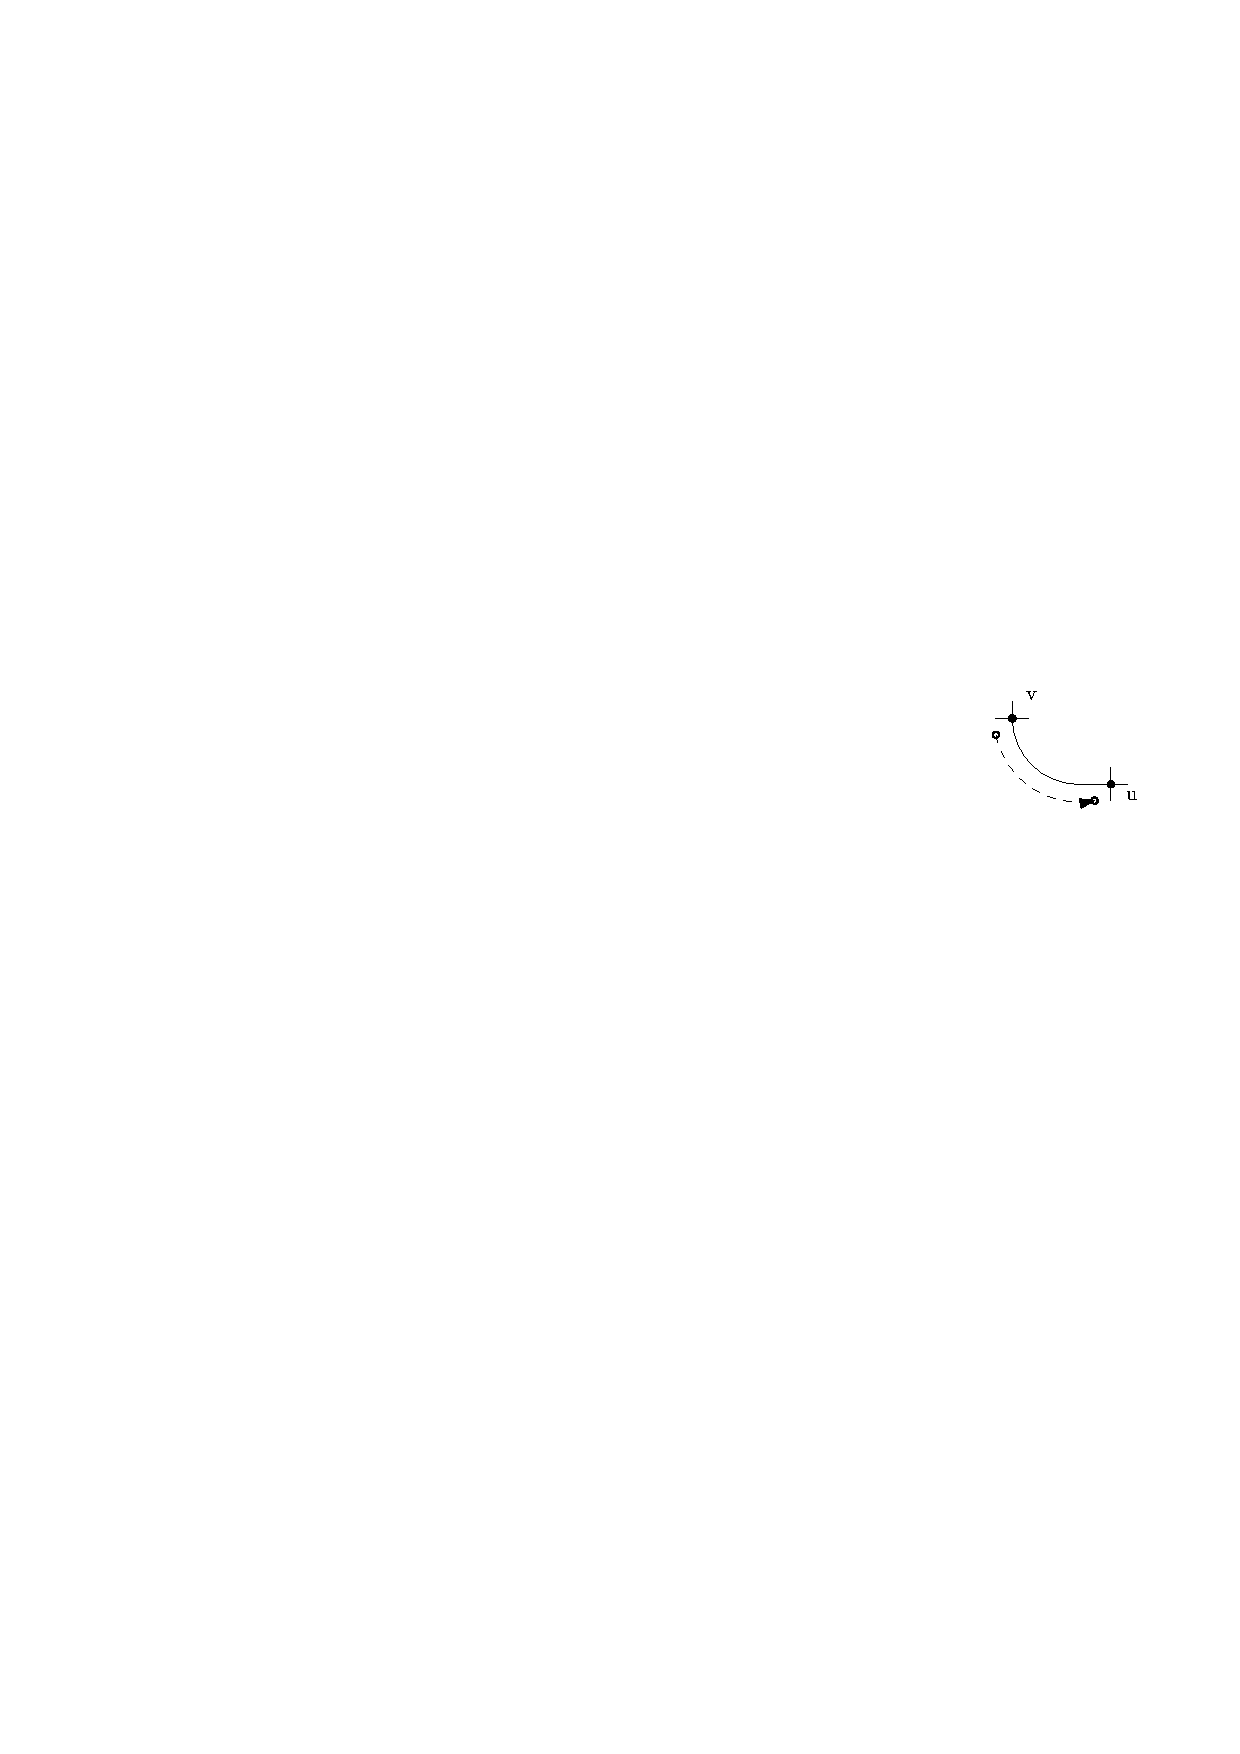
\includegraphics[width=\textwidth]{schnitt_finden_bot_belowL}
                \caption{Unterhalb, \\ unter eine \\ L-Kante}
                \label{fig:cutfinding_bot_belowL}
        \end{subfigure}
        \caption{Die verschiedenen Fälle beim Finden eines Schnitts.}\label{fig:cutfinding}
\end{figure}


Das Finden eines Schnittes durch die Zeichnung des Graphen zum Zwecke des Verschiebens von Knoten in horizontale Richtung zielt darauf ab, den Graph in zwei Teile zu spalten, die nur durch horizontale Segmente verbunden sind. 

Der Schnitt beginnt oberhalb eines Knotens, entweder knapp links oder knapp rechts davon. Er setzt sich dann durch die Zeichnung fort und folgt dabei Kanten abwärts von Knoten zu Knoten. Dabei kann er Kanten an horizontalen Segmenten durchqueren.

Hierbei ergeben sich einige verschiedene Fälle, die in Abbildung~\ref{fig:cutfinding} dargestellt sind. Hier wird jeweils der Fall, dass der Schnitt auf der linken Seite eines Knotens $v$ beginnt, betrachtet, der andere Fall wird symmetrisch behandelt. 

Soll der Schnitt leicht oberhalb eines Knotens $v$ beginnen, so muss die Kante am linken Port betrachtet werden.

Ist dort keine Kante vorhanden, kann der Schnitt direkt zur leicht unterhalb Position am gleichen Knoten $v$ fortfahren.

Ist dort eine nach oben führende Kante oder eine horizontale gerade Kante, so durchquert der Schnitt die Kante. Nach den Invarianten ist immer ein horizontales Segment an dieser Stelle. Der Schnitt verbleibt am Knoten $v$ und ist nun leicht unterhalb von $v$. Führt die Kante am linken Port nach unten, so muss es entweder eine L- oder eine C-Kante sein, in beiden Fällen folgt der Schnitt der Kante zum Zielknoten $u$. Die L-Kante endet am Zielknoten $u$ am oberen Port und der Schnitt endet links oberhalb des Zielknotens. Die C-Kante endet am Zielknoten $u$ am linken Port und der Schnitt endet links unterhalb.

Soll der Schnitt leicht unterhalb eines Knotens $v$ beginnen, so muss die Kante am unteren Port betrachtet werden. Endet die Kante an $u$ an einem rechten Port, so muss sie durchquert werden, und der Schnitt endet leicht rechts unterhalb des Zielknotens $u$. Ansonsten folgt der Schnitt der Kante. Endet die Kante an einem oberen Port, ist folglich eine gerade Kante, so endet der Schnitt leicht links oberhalb des Zielknotens. Endet die Kante an einem linken Port, liegt eine L-Kante vor und der Schnitt endet leicht links unterhalb des Zielknotens.

Für den Fall, dass der Schnitt leicht rechts eines Knotens beginnt, sind jeweils rechts und links in den Schritten und Bedingungen zu tauschen.

Nach wiederholter Anwendung dieser Regeln, wobei jeweils der Zielknoten zum neuen Ausgansknoten wird, gelangt der Schnitt schließlich zur Position leicht unterhalb eines Knotens, der keine Kante am unteren Port hat. Dies ist der unterste Knoten, und der Schnitt ist abgeschlossen.

Die Konstruktion des Schnittes speichert bei jedem Durchqueren einer Kante die Kante selbst, und den Knoten links und rechts der Kante jeweils in einer Liste von linken und rechten Knoten. Zum finden der gesamten linken Knoten wird an jedem der Knoten in der Liste der linken Knoten eine Tiefensuche begonnen, die jedoch nicht den durchschnittenen Kanten folgt. Ebenso findet man die rechten Knoten, indem man bei allen rechten Knoten startet und wiederum durchschnittene Kanten ignoriert.

\chapter{Verbesserungen}

% selten überhaupt kollisionen: 110/844

% selten muss wirklich L slope angepasst werden, macht aber viel (!!!) größer
% ohne L-slope anpassung: 1/844 collisionen

% --> use adjustments only when necessary

% keinmal mehr als 3 in einer Reihe

\chapter{Schlussfolgerungen}






\bibliographystyle{mybabalpha-fl}
\bibliography{mybib}

\end{document}
